% PREAMBLE===============================================================
\PassOptionsToPackage{table}{xcolor} % Ép mọi gói nạp sau phải dùng tùy chọn table
\documentclass[13pt,a4paper]{extarticle}
\usepackage[utf8]{inputenc}     \usepackage{textcomp}
\usepackage[left=2.5cm,right=2cm,top=2cm,bottom=2cm]{geometry}
\usepackage{times}
\usepackage{enumitem}
\usepackage{graphicx}           \usepackage{amsmath,amssymb,amsfonts}
\usepackage{algorithmic}        \usepackage{xcolor}     \usepackage{float}
\usepackage{booktabs}           \usepackage{tikz}       \usepackage[english,vietnamese]{babel}
\usepackage{multirow}           \usepackage{tabularx}   \usepackage{makecell}
\usepackage{array}
\usepackage{fancyhdr}
\usepackage{pgfplots}           \usepackage{textcomp}
\pgfplotsset{compat=1.18}
\usepackage{algorithmic}        \usepackage{balance}    \usepackage{amsmath,amssymb,amsfonts}
\usepackage{bm}                 \usepackage{url}        \usepackage{hyperref}           
\usepackage[nameinlink, noabbrev]{cleveref} 

\usetikzlibrary{shapes.geometric,arrows.meta,positioning,fit,backgrounds,calc, decorations.pathreplacing, patterns}

% ── Custom colours ───────────────────────────────────────────────────────────
\definecolor{C_slate}{RGB}{71,85,105}       \definecolor{C_blue}{RGB}{59,130,246}
\definecolor{C_indigo}{RGB}{99,102,241}     \definecolor{C_amber}{RGB}{245,158,11}
\definecolor{C_rose}{RGB}{244,63,94}        \definecolor{C_sky}{RGB}{14,165,233}
\definecolor{C_violet}{RGB}{139,92,246}     \definecolor{C_bglight}{RGB}{248,250,252}
\definecolor{C_bgmid}{RGB}{241,245,249}     \definecolor{C_emerald}{RGB}{16,185,129}
\definecolor{negcol}{RGB}{16,185,129}       \definecolor{hdrfill}{RGB}{241,245,249} 
\definecolor{C_bglight}{RGB}{248,250,252}   \definecolor{C_bgmid}{RGB}{241,245,249}
\definecolor{archblue}{RGB}{30, 58, 138}    \definecolor{archgray}{RGB}{100, 116, 139} 
\definecolor{headcol}{RGB}{30, 41, 59}    

\colorlet{hdrfill}{C_bgmid}   % Màu cho dòng tiêu đề
\colorlet{rowalt}{C_bglight}  % Màu cho dòng xen kẽ

\newcommand{\NV}{\text{NV}}
\newcommand{\TD}{\text{TD}} 
\newcommand{\BKS}{\text{BKS}}
\newcommand{\best}[1]{\textbf{\textcolor{C_emerald}{#1}}}
\newcommand{\gapneg}[1]{\textbf{\textcolor{negcol}{#1}}}

\newcommand{\tdtlogo}[1]{%
  \IfFileExists{logo-tdt.png}{%
    \includegraphics[width=#1]{logo-tdt.png}%
  }{%
    \fbox{\parbox[c][#1][c]{#1}{\centering\bfseries TDTU}}%
  }%
}

\newcommand{\procedureheader}{%
\begingroup
\fontsize{10pt}{13pt}\selectfont
\setlength{\tabcolsep}{7pt}%
\renewcommand{\arraystretch}{1.35}%
\begin{tabular}{|m{4.0cm}|m{7.0cm}|m{5.1cm}|}
\hline
\centering\vbox{\vspace{2mm}\tdtlogo{3.35cm}\vspace{2mm}} &
\textbf{\textit{Thủ tục:}}\newline\textbf{NGHIÊN CỨU KHOA HỌC SINH VIÊN} &
\raggedright\arraybackslash Mã số: TT/P.QLPTKHCN/13/BM18\newline Ban hành lần: 06\newline Ngày hiệu lực: \\
\hline
\end{tabular}%
\endgroup
}


\newcommand{\enableprocedureheader}{%
\setlength{\headheight}{104pt}%
\setlength{\headsep}{12pt}%
\fancypagestyle{procedurepages}{%
  \fancyhf{}%
  \fancyhead[C]{\makebox[0pt][c]{\procedureheader}}%
  \fancyfoot[R]{\thepage}%
  \renewcommand{\headrulewidth}{0pt}%
  \renewcommand{\footrulewidth}{0pt}%
}%
\pagestyle{procedurepages}%
}

\newcommand{\makecoverpage}{%
\onecolumn
\begin{titlepage}
\thispagestyle{empty}
\begin{tikzpicture}[remember picture, overlay]
    \draw[line width=1.5pt]
        ([shift={(1.5cm,-5.05cm)}]current page.north west)
        rectangle ([shift={(-1.2cm,1.5cm)}]current page.south east);
    \draw[line width=0.5pt]
        ([shift={(1.6cm,-5.15cm)}]current page.north west)
        rectangle ([shift={(-1.3cm,1.6cm)}]current page.south east);
\end{tikzpicture}
\noindent
\begin{center}
\makebox[0pt][c]{\procedureheader}
\end{center}
\vspace{1.15cm}
\begin{center}
    \fontsize{13pt}{16pt}\selectfont
    TỔNG LIÊN ĐOÀN LAO ĐỘNG VIỆT NAM \\
    \textbf{TRƯỜCO ĐẠI HỌC TÔN ĐỨC THẮNG} \\[0.2cm]
    ------------------------------ \\[0.35cm]

    \tdtlogo{4.8cm} \\[0.55cm]

    \fontsize{14pt}{18pt}\selectfont
    \textbf{Công trình Nghiên cứu khoa học sinh viên năm học 2025 - 2026} \\[1.45cm]

    \fontsize{19pt}{24pt}\selectfont
    \parbox{0.88\textwidth}{\centering\textbf{ỨNG DỤNG HỌC TĂNG CƯỜNG\\
    TRONG TỐI ƯU THUẬT TOÁN ALNS\\
    CHO BÀI TOÁN ĐỊNH TUYẾN XE CÓ\\
    RÀNG BUỘC KHUNG THỜI GIAN}} \\[0.65cm]
\end{center}
\noindent
\hspace{1.6cm}
\begin{minipage}{0.82\textwidth}
    \fontsize{12pt}{16pt}\selectfont
    \textbf{ĐƠN VỊ: KHOA CÔNG NGHỆ THÔNG TIN} \\[0.22cm]
    \textbf{GIẢNG VIÊN HƯỚNG DẪN:} \\
    \textit{TIẾN SĨ HỒ THỊ LINH} \\[0.22cm]
    \textbf{SINH VIÊN THỰC HIỆN:} \\[0.15cm]
    \hspace*{0.5cm} \textit{HUỲNH NHẬT HUY} --- \textit{MSSV: 523c0012}
\end{minipage}
\vfill
\begin{center}
    \fontsize{13pt}{16pt}\selectfont
    TP. Hồ Chí Minh, tháng 5 năm 2026
\end{center}
\end{titlepage}
\clearpage
}

\begin{document}
\selectlanguage{vietnamese}
\makecoverpage
\enableprocedureheader

\begin{center}
    {\bfseries\fontsize{16pt}{20pt}\selectfont TÓM TẮT CÔNG TRÌNH\par}
\end{center}

Bài toán định tuyến phương tiện có khung thời gian (Vehicle Routing Problem with Time Windows -- VRPTW) là một bài toán tối ưu hóa tổ hợp thuộc lớp NP-khó, có ý nghĩa quan trọng trong quản trị vận tải và logistics đô thị. Công trình này nghiên cứu hướng tiếp cận lai DDQN-ALNS, kết hợp Tìm kiếm lân cận lớn thích ứng (Adaptive Large Neighborhood Search -- ALNS) với Học tăng cường sâu (Deep Reinforcement Learning -- DRL), trong đó sử dụng kiến trúc Double Deep Q-Network (DDQN) và cơ chế ưu tiên lấy lại trải nghiệm (Prioritized Experience Replay -- PER) để hỗ trợ quá trình ra quyết định trong tìm kiếm lời giải.

Mô hình đề xuất được tổ chức theo hai tầng điều khiển kết hợp với các bước tối ưu hóa bổ trợ. Ở tầng chiến lược, Plateau Controller sử dụng mạng Dueling Double DQN để nhận diện trạng thái hội tụ của quá trình tìm kiếm và lựa chọn chế độ tìm kiếm phù hợp trong 6 chế độ, qua đó điều tiết quan hệ giữa khai thác (exploitation) và khám phá (exploration). Ở tầng toán tử, Operator Controller sử dụng một mạng DDQN riêng để lựa chọn cặp toán tử phá hủy và sửa chữa trong 40 tổ hợp khả dụng tại từng vòng lặp. Bên cạnh đó, cơ chế học điều kiện chấp nhận (Learned Acceptance Criterion -- LAC) được xây dựng bằng mạng nơ-ron phân loại nhị phân nhằm hỗ trợ quyết định chấp nhận lời giải ứng viên. Thuật toán cũng tích hợp Route Pool và bước tái tổ hợp tuyến đường thông qua bài toán Set Partitioning, được mô hình hóa dưới dạng Quy hoạch nguyên hỗn hợp (Mixed Integer Linear Programming -- MILP).

Kết quả thực nghiệm trên tập dữ liệu chuẩn Solomon, tập trung vào các nhóm RC1 và RC2, cho thấy DDQN-ALNS đạt độ lệch khoảng cách trung bình (Gap\%) khoảng 0.27\% ở cấu hình 1200 vòng lặp so với lời giải tốt nhất đã biết (BKS), đồng thời duy trì tiêu chí giảm số lượng phương tiện sử dụng. Trong thực nghiệm với số vòng lặp lớn (2500 vòng lặp) trên nhóm RC1, mô hình đề xuất đạt Gap\% khoảng -0.44\% (học trực tuyến) và -0.33\% (chuyển giao). Thử nghiệm chuyển giao diện rộng với ngẫu nhiên hóa miền dữ liệu (Domain Randomization) cho thấy mô hình Transfer-DR đạt Gap\% khoảng 1.62\% trên Solomon mà không cần cập nhật trọng số trực tuyến. Ngoài phần thuật toán, công trình xây dựng cổng thông tin điều phối trực quan NAMI trên nền FastAPI nhằm minh họa khả năng triển khai và hỗ trợ khai thác kết quả trong bối cảnh ứng dụng.

\clearpage
\begin{center}
    {\bfseries\fontsize{16pt}{20pt}\selectfont NỘI DUNG CÔNG TRÌNH NGHIÊN CỨU\par}
\end{center}

Trong bối cảnh kinh tế số và thương mại điện tử phát triển nhanh, dịch vụ hậu cần (logistics) giữ vai trò then chốt trong vận hành chuỗi cung ứng. Theo báo cáo của Hiệp hội Doanh nghiệp Dịch vụ Logistics Việt Nam, chi phí logistics tại Việt Nam hiện chiếm tỷ trọng khoảng 16,8\% đến 17\% GDP, cao hơn đáng kể so với mức trung bình toàn cầu. Trong số đó, chi phí vận tải đường bộ chiếm tới hơn 60\% tổng chi phí logistics. Thực trạng này đặt ra yêu cầu tối ưu hóa lộ trình vận chuyển nhằm tiết kiệm nhiên liệu, rút ngắn thời gian giao hàng, giảm số lượng phương tiện sử dụng và hỗ trợ doanh nghiệp nâng cao hiệu quả vận hành.

Bài toán định tuyến phương tiện có khung thời gian (Vehicle Routing Problem with Time Windows -- VRPTW) là mô hình toán học phản ánh trực tiếp thách thức thực tế này. Trong VRPTW, một đội xe xuất phát từ một kho chứa trung tâm cần phục vụ một tập hợp khách hàng phân tán về địa lý. Mỗi khách hàng có nhu cầu hàng hóa xác định và yêu cầu phục vụ trong một khung thời gian cụ thể. Nếu xe đến trước thời điểm cho phép, phương tiện phải chờ; nếu đến sau giới hạn thời gian, phương án tuyến bị xem là vi phạm ràng buộc. VRPTW thuộc lớp bài toán NP-khó (NP-hard), nghĩa là thời gian tìm kiếm lời giải tối ưu toán học sẽ tăng lên theo hàm mũ khi số lượng khách hàng tăng lên.

Mặc dù các thuật toán heuristic và meta-heuristic, tiêu biểu là Tìm kiếm lân cận lớn thích ứng (ALNS), đã cho thấy hiệu quả trong nhiều bài toán kích thước trung bình và lớn, hiệu năng của chúng vẫn phụ thuộc đáng kể vào cách thiết lập tham số và cơ chế điều khiển được thiết kế thủ công. Sự kết hợp giữa các kỹ thuật học máy hiện đại, đặc biệt là Học tăng cường sâu (DRL), mở ra một hướng tiếp cận đáng nghiên cứu. DRL cho phép hệ thống tự học các chiến lược chọn toán tử tối ưu và tự động điều phối trạng thái tìm kiếm dựa trên kinh nghiệm tích lũy từ các vòng lặp trước đó.

Từ các phân tích trên, đề tài ``Ứng dụng học tăng cường trong tối ưu thuật toán ALNS cho bài toán định tuyến xe có ràng buộc khung thời gian'' được thực hiện nhằm xây dựng một phương pháp tối ưu hóa có khả năng xử lý ràng buộc khung thời gian, ưu tiên giảm quy mô đội xe và đánh giá khả năng ứng dụng trong bài toán logistics tại Việt Nam.

\clearpage
\section{Tổng quan tài liệu}

Bài toán định tuyến phương tiện (VRP) được giới thiệu lần đầu bởi Dantzig và Ramser (1959). Kể từ đó, hàng loạt biến thể của bài toán đã được phát triển nhằm đáp ứng các yêu cầu thực tiễn, trong đó VRPTW là biến thể phổ biến nhất do tính thực tế cao của các ràng buộc về mặt thời gian (Solomon, 1987).

Để giải quyết VRPTW, phương pháp tiếp cận trọng lịch sử được chia làm ba nhóm chính:

\textbf{Phương pháp chính xác (Exact Methods):} Sử dụng các thuật toán như Quy hoạch động (Dynamic Programming), Nhánh và Cắt (Branch and Cut), hay Nhánh-Giá và Cắt (Branch-and-Price-and-Cut). Mặc dù các phương pháp này đảm bảo tìm ra lời giải tối ưu toàn cục, chúng gặp hạn chế lớn về khả năng mở rộng (scalability). Khi số lượng khách hàng vượt quá 100, thời gian tính toán tăng lên đến hàng giờ hoặc hàng ngày, khiến chúng không thể áp dụng cho các bài toán điều phối thời gian thực trong doanh nghiệp.

\textbf{Phương pháp Heuristic và Meta-heuristic:} Để đánh đổi độ tối ưu tuyệt đối lấy thời gian tính toán nhanh, các thuật toán tìm kiếm metaheuristic như Giải thuật Di truyền (Genetic Algorithm), Tối ưu hóa bầy đàn (Particle Swarm Optimization), hay Tìm kiếm Tabu (Tabu Search) đã được áp dụng rộng rãi. Đặc biệt, thuật toán Tìm kiếm lân cận lớn thích ứng (ALNS), được đề xuất bởi Ropke và Pisinger (2006), đã trở thành chuẩn mực công nghiệp để giải quyết các bài toán định tuyến quy mô lớn. ALNS hoạt động bằng cách liên tục phá hủy một phần lời giải hiện tại và tái thiết nó bằng các toán tử sửa chữa khác nhau dưới sự điều phối của thuật toán roulette wheel hoặc Thompson Bandit. Tuy nhiên, hạn chế lớn nhất của ALNS là cơ chế cập nhật trọng số toán tử có độ trễ lớn và chỉ dựa trên thống kê tần suất cục bộ, không thể nhận biết được sự thay đổi phức tạp của không gian trạng thái tìm kiếm ở các giai đoạn hội tụ khác nhau. Đồng thời, việc sử dụng tiêu chuẩn Simulated Annealing để chấp nhận lời giải ứng viên phụ thuộc nặng nề vào tham số nhiệt độ ban đầu và hệ số làm nguội cứng nhắc, dễ dẫn đến việc thuật toán bị kẹt trong các cực trị địa phương (local optima) hoặc hội tụ non.

\textbf{Phương pháp Học máy và Học tăng cứu sâu (DRL):} Trong những năm gần đây, xu hướng ứng dụng mạng nơ-ron để học cách giải quyết các bài toán tối ưu hóa tổ hợp phát triển mạnh mẽ. Kool và đồng tác giả (2018) đã đề xuất mô hình Attention Model để giải VRP trực tiếp dưới dạng mô hình end-to-end. Tuy nhiên, các phương pháp end-to-end thuần túy thường gặp khó khăn khi đối mặt với các ràng buộc cứng ngặt nghèo của khung thời gian (Time Windows) và khó tổng quát hóa khi quy mô bài toán thay đổi. Hướng tiếp cận lai (Hybrid) -- kết hợp DRL để đưa ra các quyết định chiến lược cấp cao và meta-heuristic để thực hiện tìm kiếm cấu trúc tuyến đường cấp thấp -- đang là hướng nghiên cứu được quan tâm. Kỹ thuật này giúp tận dụng khả năng học biểu diễn và ra quyết định của mạng thần kinh nhân tạo mà vẫn đảm bảo tính hợp lệ của lời giải thông qua các toán tử heuristic.

Trong nghiên cứu này, nhóm tác giả đề xuất mô hình lai \textbf{DDQN-ALNS} nhằm cải thiện các hạn chế trên thông qua các thành phần sau:
\begin{itemize}[leftmargin=1.2cm]
  \item Thiết lập bộ điều khiển cấp cao Plateau Controller để chuyển đổi linh hoạt 6 chế độ tìm kiếm khác nhau dựa trên các đặc trưng động lực học tiến trình.
  \item Thiết lập bộ điều khiển cấp thấp Operator Controller tích hợp cơ chế UCB và Thompson Bandit để nâng cao tính khám phá của các cặp toán tử.
  \item Thay thế tiêu chuẩn Simulated Annealing truyền thống bằng mạng thần kinh phân loại nhị phân học điều kiện chấp nhận (LAC).
  \item Kết hợp công cụ quy hoạch toán học MILP giải bài toán Set Partitioning trên Route Pool để định kỳ tái cấu trúc lời giải tối ưu.
\end{itemize}

\subsection{Phân tích khoảng trống nghiên cứu (Gap Analysis)}

Mặc dù các hướng tiếp cận học máy và meta-heuristic lai đã đạt được một số thành tựu nhất định, nghiên cứu này xác định ba khoảng trống công nghệ chính từ các nghiên cứu đi trước và đề xuất phương án khắc phục cụ thể:

\textbf{So với Hottung và Tierney (2020) \cite{hottung2020}:}
Phương pháp \textit{Neural Large Neighborhood Search (NLNS)} của Hottung \& Tierney \cite{hottung2020} hoặc giải thuật \textit{Deep Policy Dynamic Programming (DPDP)} của Kool và cộng sự (2021) \cite{kool2021} tập trung vào việc sử dụng mạng thần kinh (attention-based hoặc GNN) để trực tiếp sinh lộ trình, sinh quyết định phá hủy/sửa chữa ở cấp độ nút (node-level) hoặc lọc không gian trạng thái. Tuy nhiên, hướng tiếp cận sinh trực tiếp này gặp khó khăn rất lớn khi đối mặt với các bài toán có ràng buộc khung thời gian cứng và ngặt nghèo (Time Windows) do không gian lời giải hợp lệ bị co hẹp đáng kể, dẫn đến việc mạng nơ-ron dễ sinh ra các lộ trình không khả thi hoặc tốn kém thời gian sửa đổi. Ngược lại, mô hình lai \textbf{DDQN-ALNS} đề xuất sử dụng DRL ở cấp độ điều khiển chiến lược (chọn chế độ tìm kiếm và chọn cặp toán tử heuristic từ thư viện có sẵn). Việc giữ nguyên các toán tử sửa chữa heuristic giúp đảm bảo tính khả thi tuyệt đối của lời giải về mặt toán học thông qua các bộ lọc ràng buộc nhanh, trong khi vẫn tận dụng được khả năng học hỏi thông minh từ mạng nơ-ron để tăng tốc độ hội tụ.

\textbf{So với Bi và đồng tác giả (2022) \cite{bi2022}:}
Bi et al. \cite{bi2022} đề xuất giải pháp L-ALNS sử dụng một tác nhân học tăng cường duy nhất để chọn toán tử và dựa trên tiêu chuẩn Simulated Annealing (SA) truyền thống để chấp nhận lời giải. Điểm hạn chế là tác nhân chọn toán tử không nhận biết được các giai đoạn hội tụ khác nhau của tiến trình tìm kiếm tổng thể và tiêu chuẩn SA phụ thuộc quá nhiều vào bộ tham số nhiệt độ cứng nhắc. Mô hình đề xuất của chúng tôi khắc phục điều này bằng kiến trúc \textit{học phân cấp hai cấp độ} (Plateau Controller cho chế độ tìm kiếm ở cấp chiến lược phân đoạn, Operator Controller ở cấp vòng lặp) kết hợp với mạng phân loại học điều kiện chấp nhận (LAC) thay thế hoàn toàn SA, và cơ chế tái tổ hợp Set Partitioning tối ưu hóa chính xác bằng MILP.

\textbf{So với các phương pháp Heuristic điều hướng bằng LLM (LLM-driven Heuristics):}
Một số nghiên cứu gần đây sử dụng mô hình ngôn ngữ lớn (LLM) để tìm kiếm và sinh mã nguồn cho các toán tử heuristic như VRPAgent \cite{vrpagent2024} hay MEP \cite{mep2024}. Các phương pháp này thực chất là quá trình tối ưu hóa ngoại tuyến (offline optimization/refinement), sinh ra một thuật toán tĩnh trước khi giải bài toán. Trái lại, giải thuật \textbf{DDQN-ALNS} của chúng tôi là một mô hình học trực tuyến (online decision maker). Nó liên tục đánh giá trạng thái động của tiến trình tối ưu hóa và đưa ra quyết định hành động thích ứng thời gian thực (real-time adaptive control) ngay trong quá trình giải một thực thể cụ thể, điều mà các phương pháp sinh mã tĩnh bằng LLM không thể thực hiện được.

\clearpage
\section{Mục tiêu -- Phương pháp}
\subsection{Mục tiêu nghiên cứu}

Mục tiêu tổng quát của đề tài là xây dựng và đánh giá một phương pháp tối ưu hóa lai giữa Tìm kiếm lân cận lớn thích ứng (ALNS) và Học tăng cường sâu (DRL) cho bài toán định tuyến phương tiện có khung thời gian (VRPTW). Phương pháp hướng đến việc tìm lời giải khả thi có chất lượng cao, ưu tiên giảm số lượng phương tiện sử dụng, giảm tổng quãng đường di chuyển và duy trì khả năng xử lý hiệu quả trên các bộ dữ liệu chuẩn cũng như trong bối cảnh ứng dụng logistics thực tế.

Các mục tiêu cụ thể của nghiên cứu bao gồm:
\begin{itemize}[leftmargin=1.2cm]
  \item Thiết lập đặc tả toán học đầy đủ cho bài toán VRPTW trên đồ thị định hướng, bao gồm tập khách hàng, kho trung tâm, sức tải phương tiện, nhu cầu hàng hóa, thời gian phục vụ, thời gian di chuyển và ràng buộc khung thời gian.
  \item Xây dựng hàm mục tiêu phân cấp, trong đó ưu tiên tối thiểu hóa số lượng xe vận hành trước, sau đó tối thiểu hóa tổng quãng đường hoặc tổng chi phí di chuyển nhằm phản ánh đúng yêu cầu kinh tế của bài toán logistics.
  \item Thiết kế thuật toán lai DDQN-ALNS, kết hợp khả năng phá hủy--sửa chữa lời giải của ALNS với năng lực học chính sách điều khiển của mạng Dueling Double Deep Q-Network.
  \item Phát triển bộ điều khiển cấp cao Plateau Controller để nhận diện trạng thái hội tụ của quá trình tìm kiếm và tự động lựa chọn chế độ tìm kiếm phù hợp giữa khai thác và khám phá.
  \item Phát triển bộ điều khiển cấp thấp Operator Controller để lựa chọn cặp toán tử phá hủy và sửa chữa hiệu quả tại từng vòng lặp, có xét đến lịch sử cải thiện lời giải và trạng thái hiện tại của thuật toán.
  \item Đề xuất cơ chế học điều kiện chấp nhận lời giải (Learned Acceptance Criterion -- LAC) nhằm thay thế hoặc bổ trợ tiêu chuẩn Simulated Annealing truyền thống, qua đó cải thiện khả năng vượt qua cực trị địa phương.
  \item Tích hợp Route Pool và mô hình Set Partitioning để tái tổ hợp các tuyến đường chất lượng cao, hỗ trợ cải thiện lời giải sau các giai đoạn tìm kiếm cục bộ.
  \item Thực nghiệm và so sánh thuật toán đề xuất trên bộ dữ liệu chuẩn Solomon, sử dụng các tiêu chí số lượng xe, tổng quãng đường, độ lệch so với lời giải tốt nhất đã biết và thời gian tính toán.
  \item Đánh giá khả năng chuyển giao của mô hình thông qua ngẫu nhiên hóa miền dữ liệu, nhằm kiểm tra mức độ thích ứng của chính sách học tăng cường khi gặp các thực thể mới.
  \item Xây dựng hệ thống trực quan hóa và hỗ trợ điều phối tuyến đường, cho phép minh họa kết quả thuật toán và định hướng khả năng triển khai trong môi trường doanh nghiệp.
\end{itemize}

\subsection{Đặc tả toán học bài toán VRPTW}

Bài toán được phát biểu trên đồ thị định hướng đầy đủ $G = (V, A)$. Đội xe đồng nhất gồm $K$ phương tiện, mỗi phương tiện có sức tải tối đa $Q$. Các ký hiệu và biến quyết định được mô tả như sau:

\vspace{0.10cm}
\begin{figure}[H]
\centering
\resizebox{0.98\textwidth}{!}{%
\begin{tikzpicture}[every node/.style={font=\small}]
  \tikzset{
    depot/.style={rectangle, rounded corners=2pt, draw=headcol, fill=C_bgmid, thick, minimum width=0.95cm, minimum height=0.55cm},
    customer/.style={circle, draw=C_blue!75!black, fill=C_blue!8, thick, minimum size=0.58cm, inner sep=0pt},
    routeA/.style={-{Latex[length=2mm]}, thick, C_blue!80!black},
    routeB/.style={-{Latex[length=2mm]}, thick, C_emerald!75!black, dashed},
    twbar/.style={draw=C_slate!60, fill=C_bgmid, rounded corners=1pt, line width=0.45pt},
    service/.style={draw=C_rose!80!black, fill=C_rose!35, rounded corners=1pt, line width=0.45pt},
    grid/.style={C_slate!16, line width=0.25pt},
    note/.style={font=\scriptsize, text=C_slate}
  }

  \node[font=\bfseries\small, text=headcol] at (2.70,2.05) {(a) Tuyến xe và khách hàng};
  \node[depot] (d) at (0,0) {Kho};
  \node[customer] (c1) at (1.30,0.92) {$1$};
  \node[customer] (c2) at (2.80,1.10) {$2$};
  \node[customer] (c3) at (4.05,0.35) {$3$};
  \node[customer] (c4) at (1.40,-0.98) {$4$};
  \node[customer] (c5) at (3.25,-1.10) {$5$};

  \draw[routeA] (d) -- (c1);
  \draw[routeA] (c1) -- (c2);
  \draw[routeA] (c2) -- (c3);
  \draw[routeA] (c3) to[bend left=10] (d);
  \draw[routeB] (d) -- (c4);
  \draw[routeB] (c4) -- (c5);
  \draw[routeB] (c5) to[bend right=10] (d);

  \draw[routeA] (4.80,0.70) -- ++(0.60,0) node[right, note] {Tuyến xe 1};
  \draw[routeB] (4.80,0.20) -- ++(0.60,0) node[right, note] {Tuyến xe 2};

  \begin{scope}[xshift=7.25cm, yshift=-0.05cm, xscale=1.05]
    \node[font=\bfseries\small, text=headcol] at (3.15,2.10) {(b) Chiều thời gian và khung phục vụ};
    \foreach \x/\lab in {0/0,1/2,2/4,3/6,4/8,5/10} {
      \draw[grid] (\x,-1.25) -- (\x,1.25);
      \node[font=\scriptsize, text=C_slate] at (\x,-1.48) {\lab};
    }
    \draw[-{Latex[length=2mm]}, C_slate, line width=0.65pt] (0,-1.25) -- (5.35,-1.25) node[right, font=\scriptsize] {$t$};

    \foreach \y/\name/\start/\len/\srv in {1.05/1/0.35/1.85/0.95,0.50/2/1.10/1.80/1.75,-0.05/3/2.15/1.55/2.75,-0.60/4/0.70/1.70/1.18,-1.15/5/2.85/1.45/3.50} {
      \node[left, font=\scriptsize, text=headcol] at (-0.14,\y+0.10) {$KH_{\name}$};
      \draw[twbar] (\start,\y) rectangle ++(\len,0.20);
      \draw[service] (\srv,\y-0.035) rectangle ++(0.32,0.27);
    }
    \draw[twbar] (5.85,0.35) rectangle ++(0.38,0.14);
    \node[right, note] at (6.32,0.42) {$[E_i,L_i]$};
    \draw[service] (5.85,-0.20) rectangle ++(0.30,0.18);
    \node[right, note] at (6.32,-0.11) {thời điểm phục vụ};
  \end{scope}
\end{tikzpicture}%
}
\caption{Minh họa bài toán VRPTW: tuyến xe trong không gian khách hàng và ràng buộc khung thời gian phục vụ trên trục thời gian.}
\label{fig:vrptw_clean}
\end{figure}
\clearpage
\begin{itemize}[leftmargin=1.2cm]
  \item $q_i$: nhu cầu hàng hóa của khách hàng $i \in C = \{1, 2, \dots, n\}$.
  \item $s_i$: thời gian phục vụ tại đỉnh $i$.
  \item $[E_i, L_i]$: khung thời gian bắt đầu phục vụ tại đỉnh $i$.
  \item $d_{ij}$: khoảng cách di chuyển từ đỉnh $i$ sang đỉnh $j$.
  \item $t_{ij}$: thời gian di chuyển từ đỉnh $i$ sang đỉnh $j$.
  \item $x_{ijk} \in \{0, 1\}$: bằng 1 nếu xe $k$ di chuyển từ $i$ sang $j$, ngược lại bằng 0.
  \item $w_{ik}$: thời điểm xe $k$ bắt đầu phục vụ tại đỉnh $i$.
\end{itemize}

Công thức hóa quy hoạch tuyến tính nguyên hỗn hợp (MILP) được sử dụng như sau:

\textbf{Hàm mục tiêu:}
\begin{equation}
\min \quad f(x) = M \cdot \sum_{k \in K} \sum_{j \in C} x_{0jk} + \sum_{k \in K} \sum_{(i, j) \in A} d_{ij} x_{ijk}
\end{equation}
\vspace{0.12cm}

Với hằng số phạt xe $M \gg \sum_{(i, j) \in A} d_{ij}$.

\textbf{Hệ thống các ràng buộc chính:}

\noindent\textit{(i) Ràng buộc phục vụ khách hàng:} mỗi khách hàng được phục vụ đúng một lần bởi một phương tiện.
\begin{equation}
\sum_{k \in K} \sum_{j \in V \setminus \{0\}} x_{ijk} = 1, \quad \forall i \in C
\end{equation}

\noindent\textit{(ii) Ràng buộc xuất phát và kết thúc tuyến:} mỗi xe nếu được sử dụng chỉ rời kho tối đa một lần và quay về điểm kết thúc tối đa một lần.
\begin{align}
\sum_{j \in V \setminus \{0\}} x_{0jk} &\le 1, \quad \forall k \in K \\
\sum_{i \in V \setminus \{n+1\}} x_{i,n+1,k} &\le 1, \quad \forall k \in K
\end{align}

\noindent\textit{(iii) Ràng buộc bảo toàn luồng:} nếu xe đi vào một khách hàng thì cũng phải rời khỏi khách hàng đó.
\begin{equation}
\sum_{i \in V} x_{ijk} - \sum_{i' \in V} x_{ji'k} = 0, \quad \forall j \in C, \forall k \in K
\end{equation}

\noindent\textit{(iv) Ràng buộc tải trọng:} tổng nhu cầu trên tuyến của mỗi xe không vượt quá sức tải $Q$.
\begin{equation}
\sum_{i \in C} q_i \sum_{j \in V} x_{ijk} \le Q, \quad \forall k \in K
\end{equation}

\noindent\textit{(v) Ràng buộc thời gian và khung phục vụ:} thời điểm phục vụ phải tôn trọng thứ tự di chuyển và nằm trong khung $[E_i,L_i]$.
\begin{align}
w_{ik} + s_i + t_{ij} - M_{ij} (1 - x_{ijk}) &\le w_{jk}, \quad \forall (i, j) \in A, \forall k \in K \\
E_i \le w_{ik} &\le L_i, \quad \forall i \in V, \forall k \in K
\end{align}

\noindent\textit{(vi) Miền giá trị biến quyết định:} biến cung nhận giá trị nhị phân.
\begin{equation}
x_{ijk} \in \{0, 1\}, \quad \forall (i, j) \in A, \forall k \in K
\end{equation}
\clearpage
\subsection{Phương pháp nghiên cứu đề xuất (Hybrid DDQN-ALNS)}
\subsubsection{Kiến trúc tổng quan hệ thống}

Kiến trúc đề xuất tích hợp một quy trình lặp tuần hoàn kết hợp DRL và MILP như Hình~\ref{fig:hybrid_ddqn_alns_arch}.

\begin{figure}[H]
\centering
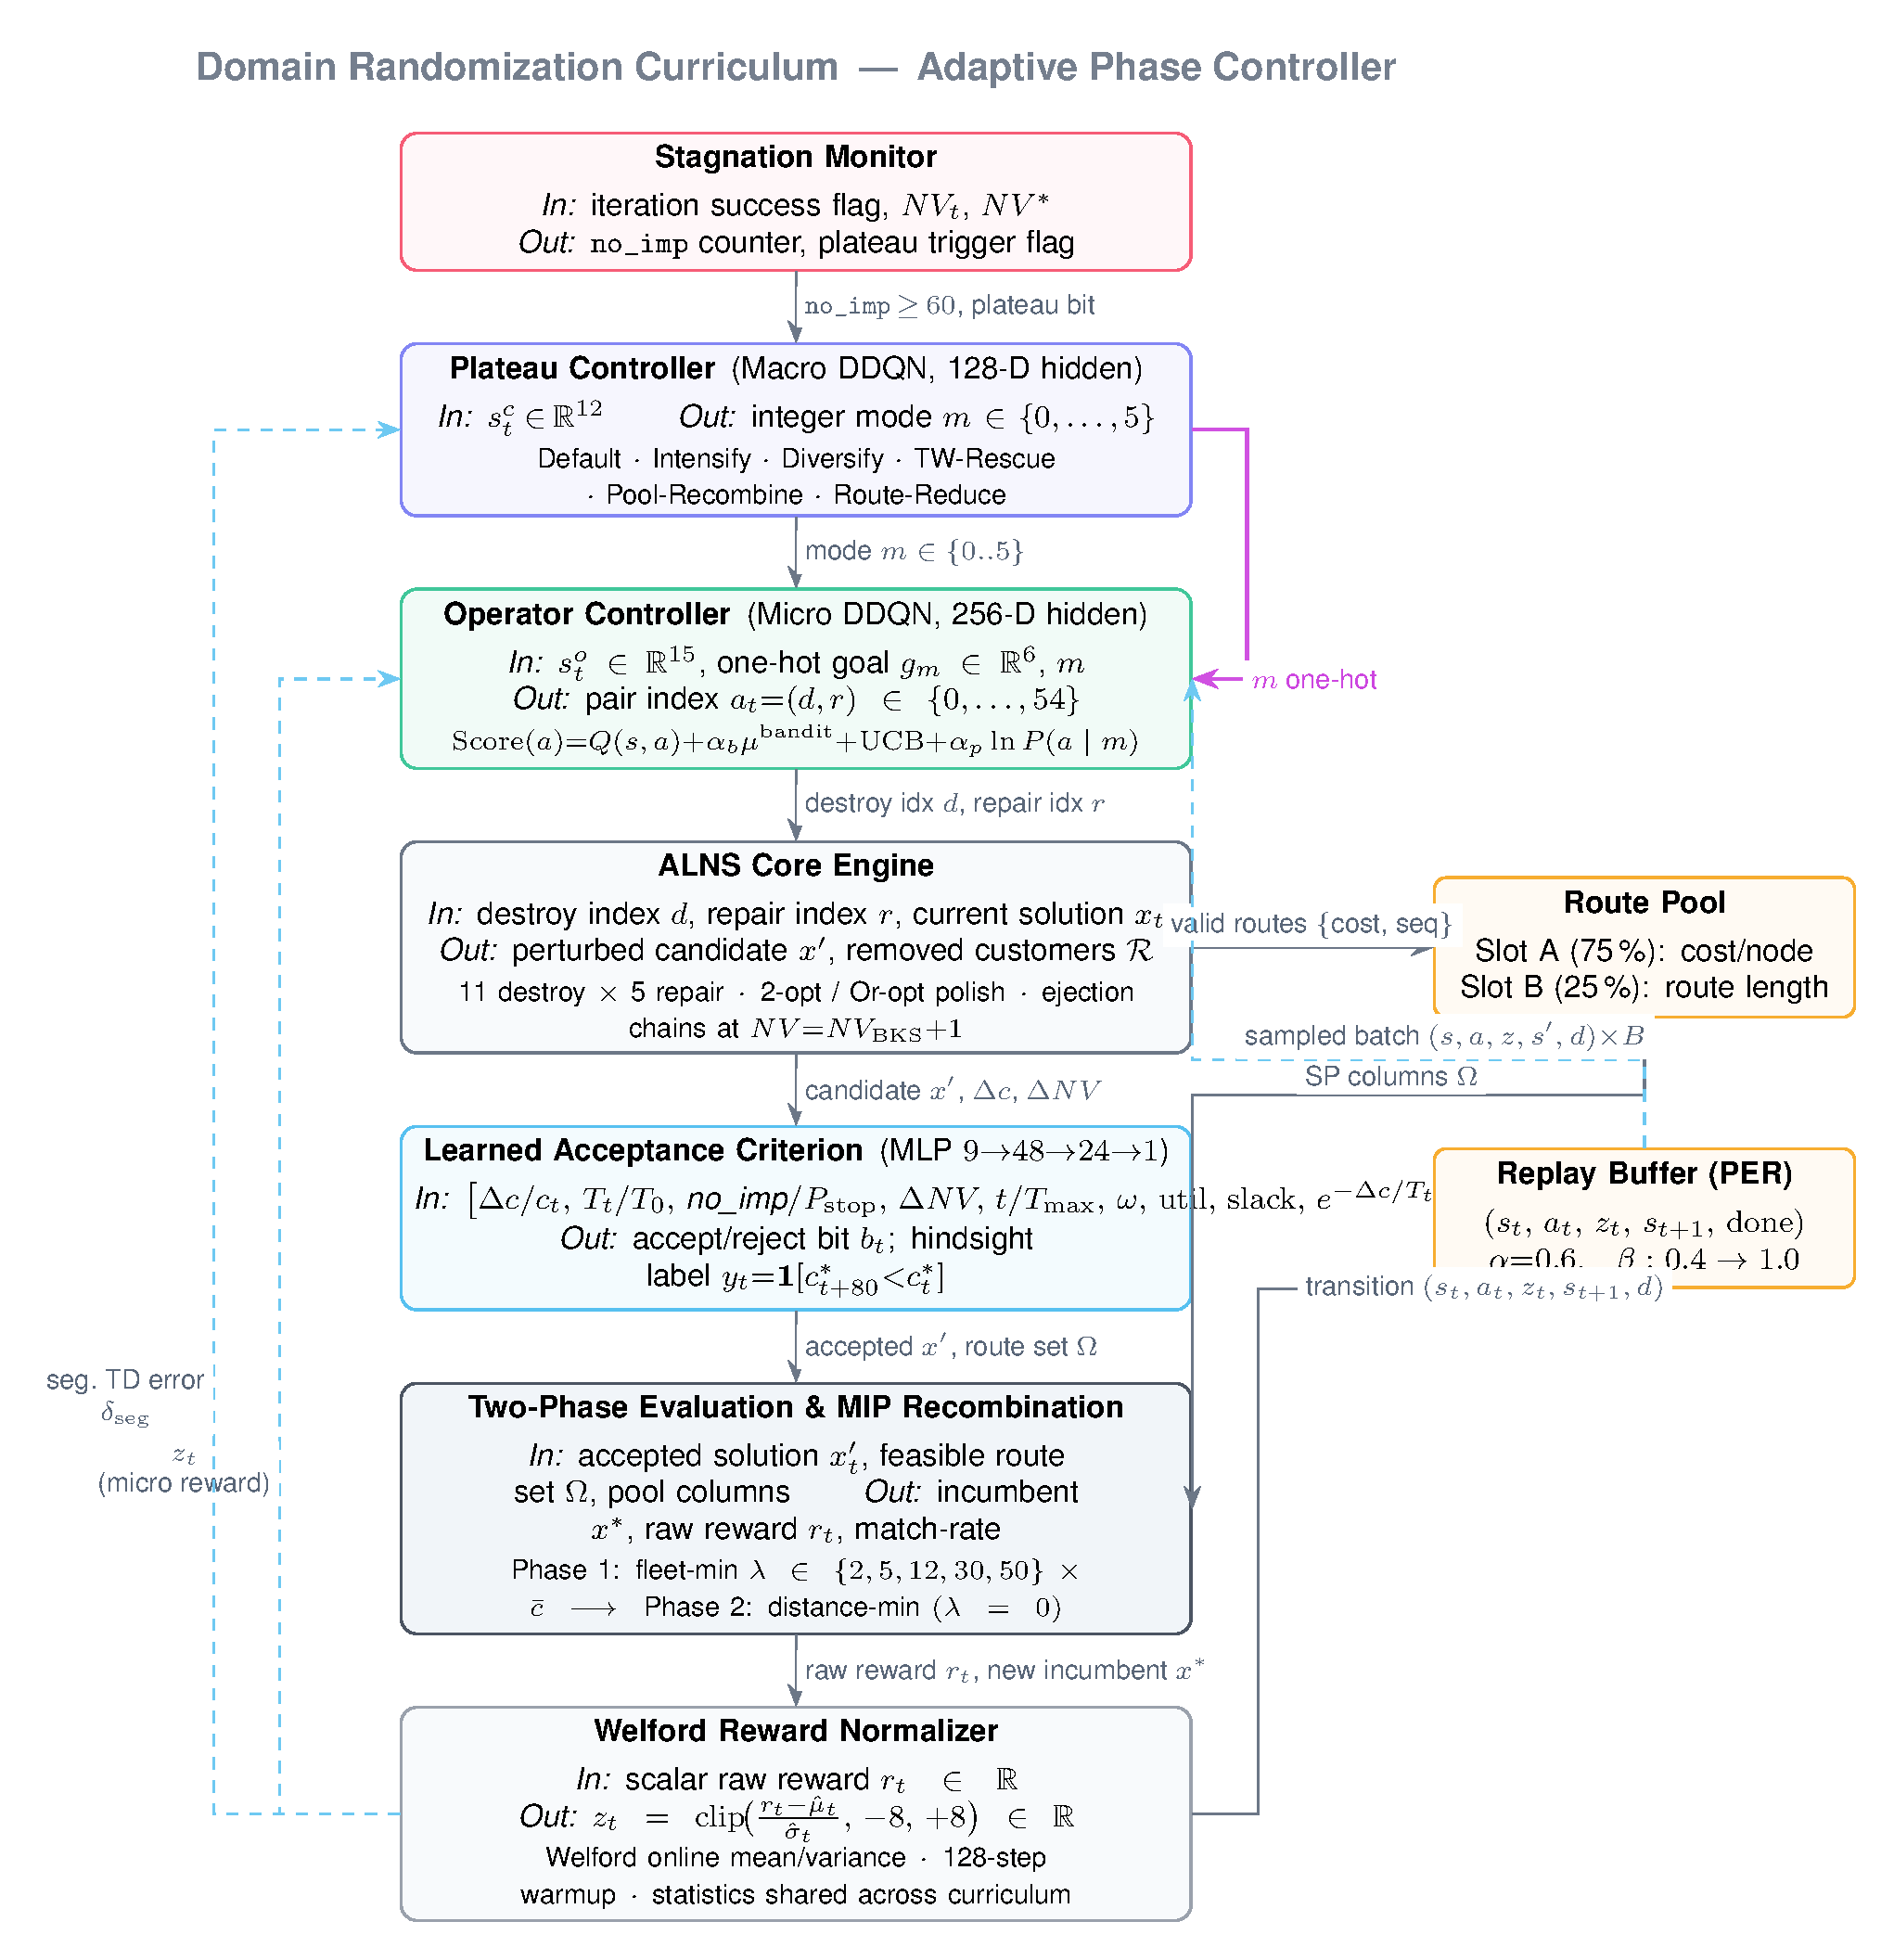
\includegraphics[width=0.62\textwidth,height=0.40\textheight,keepaspectratio]{hybrid-ddqn-alns-model-full.png}
\caption{Kiến trúc Hierarchical MDP temporally-coupled của hệ thống Hybrid DDQN-ALNS, kết hợp Plateau Controller, Operator Controller, ALNS Core Engine, LAC và Welford Normalizer trong một vòng lặp học--tối ưu. Ký hiệu luồng: Mũi tên liền nét (luồng dữ liệu tiến), Mũi tên đứt nét màu xanh (vòng phản hồi phần thưởng), Mũi tên màu hồng/magenta (vector chế độ điều phối mục tiêu).}
\label{fig:hybrid_ddqn_alns_arch}
\end{figure}

\begin{enumerate}[leftmargin=1.2cm]
  \item Bắt đầu: Khởi tạo lời giải $S_{init}$.
  \item Phân đoạn mới: $t = segment\_size$.
  \item Plateau Controller nhận vector $s_{12}$ và chọn Search Mode.
  \item Vòng lặp ALNS bên trong.
  \item Operator Controller nhận vector $s_{15}$ và chọn Destroyer/Repairer.
  \item Áp dụng cặp toán tử phá hủy và sửa chữa.
  \item LAC đánh giá chấp nhận lời giải ứng viên $S_{new}$.
  \item Nếu chấp nhận: cập nhật $S_{current}=S_{new}$ và thêm tuyến vào Route Pool; nếu từ chối: giữ nguyên $S_{current}$.
  \item Kiểm tra hết phân đoạn; nếu chưa, quay lại vòng lặp ALNS bên trong.
  \item Định kỳ, nếu bật $pool\_recombine$, giải Set Partitioning qua MILP bằng SciPy Solver.
  \item Áp dụng Local Search và giải thuật giảm xe chủ động.
  \item Kiểm tra tiêu chuẩn dừng; nếu chưa thỏa, bắt đầu phân đoạn mới; nếu thỏa, trả về lời giải tối ưu $S_{best}$.
\end{enumerate}
\normalsize

Tiến trình hoạt động của thuật toán lai DDQN-ALNS được mô tả hình thức thông qua mã giả tại Thủ tục 1 dưới đây:

\begingroup
\fontsize{11pt}{14pt}\selectfont
\begin{tabbing}
\textbf{Thủ tục 1:} Quy trình thực thi tuần hoàn của thuật toán lai Hybrid DDQN-ALNS \\
\rule{\linewidth}{0.4pt}
\textbf{Đầu vào:} Thực thể VRPTW $I$, cấu hình $CFG$, các mạng thần kinh ($Q_{plat}$, $Q_{op}$, $Net_{lac}$)\\
\textbf{Đầu ra:} Lời giải tối ưu toàn cục $S_{best}$\\
1. Khởi tạo lời giải ban đầu khả thi $S_{init}$ bằng Heuristic Greedy Insertion; \\
2. $S_{cur} \leftarrow S_{init}$; $S_{best} \leftarrow S_{init}$; $\mathcal{P} \leftarrow \{r \mid r \in S_{init}\}$ (Route Pool); \\
3. Khởi tạo Thompson Bandit $B$, bộ tăng cường $UCB$, và chuẩn hóa Welford $N_{norm}$; \\
4. Đặt $T \leftarrow T_{init}$; $no\_imp \leftarrow 0$; $Mode \leftarrow default$; $t \leftarrow 0$; \\
5. \textbf{While} $t < CFG.max\_iterations$ \textbf{and} $no\_imp < CFG.early\_stop\_patience$ \textbf{do} \\
6. \qquad \textbf{If} $t > 0$ \textbf{and} $t \pmod{CFG.segment\_size} == 0$ \textbf{then} \\
7. \qquad\qquad Trích xuất vector trạng thái chiến lược $s_{plat} \in \mathbb{R}^{12}$; \\
8. \qquad\qquad Chọn hành động chế độ: $Mode \leftarrow \text{argmax}_{a} Q_{plat}(s_{plat}, a)$; \\
9. \qquad\qquad Cập nhật tham số ALNS ($\alpha_{dest}$, $\alpha_{decay}$, Local Search) theo hành động $Mode$; \\
10. \qquad \textbf{EndIf} \\
11. \qquad Trích xuất vector trạng thái cấp thấp $s_{op} \in \mathbb{R}^{15}$; \\
12. \qquad Dự đoán giá trị Q-network: $Q^{net} \leftarrow Q_{op}(s_{op})$; \\
13. \qquad Augment điểm số: $Q^{final} \leftarrow Q^{net} + \theta_{prior} \ln(P^{prior}) + \theta_{bandit} P^{bandit} + \theta_{ucb} UCB$; \\
14. \qquad Chọn cặp toán tử phá hủy và sửa chữa: $(d, r) \leftarrow \text{divmod}(\text{argmax}(Q^{final}), 5)$; \\
15. \qquad Phá hủy $q$ khách hàng từ $S_{cur}$ bằng $d$, rồi sửa chữa chèn lại bằng $r \to S_{new}$; \\
16. \qquad Trích xuất vector đặc trưng chấp nhận $s_{lac} \in \mathbb{R}^9$; \\
17. \qquad Tính xác suất chấp nhận $p_{accept} \leftarrow Net_{lac}(s_{lac})$; \\
18. \qquad \textbf{If} $\text{Random}(0, 1) < p_{accept}$ \textbf{then} \\
19. \qquad\qquad $S_{cur} \leftarrow S_{new}$; Thêm mọi tuyến thuộc $S_{new}$ vào Route Pool $\mathcal{P}$; \\
20. \qquad \textbf{EndIf} \\
21. \qquad \textbf{If} $f(S_{new}) < f(S_{best})$ \textbf{then} \\
22. \qquad\qquad $S_{best} \leftarrow S_{new}$; $no\_imp \leftarrow 0$; \\
23. \qquad \textbf{Else} \\
24. \qquad\qquad $no\_imp \leftarrow no\_imp + 1$; \\
25. \qquad \textbf{EndIf} \\
26. \qquad \textbf{If} $Mode == pool\_recombine$ \textbf{and} $t \pmod{\text{period}} == 0$ \textbf{then} \\
27. \qquad\qquad Giải bài toán Set Partitioning trên Route Pool $\mathcal{P}$ qua MILP (SciPy, giới hạn 4.0s) $\to S_{milp}$; \\
28. \qquad\qquad \textbf{If} Tìm thấy lời giải hợp lệ $S_{milp}$ \textbf{then} \\
29. \qquad\qquad\qquad $S_{cur} \leftarrow S_{milp}$; \textbf{If} $f(S_{milp}) < f(S_{best})$ \textbf{then} $S_{best} \leftarrow S_{milp}$; $no\_imp \leftarrow 0$; \textbf{EndIf} \\
30. \qquad\qquad \textbf{EndIf} \\
31. \qquad \textbf{EndIf} \\
32. \qquad \textbf{If} Kích hoạt Local Search (2-opt, Swap, Relocate, Cross-Exchange) hoặc giảm xe chủ động \textbf{then} \\
33. \qquad\qquad Thực hiện cải thiện cục bộ trên $S_{cur}$; Cập nhật lại $S_{best}$ nếu có cải thiện; \\
34. \qquad \textbf{EndIf} \\
35. \qquad Cập nhật Thompson Bandit $B$, UCB, và Normalizer $N_{norm}$ theo điểm số chênh lệch thực tế; \\
36. \qquad Cập nhật nhiệt độ $T \leftarrow T \times \alpha_{decay}$; $t \leftarrow t + 1$; \\
37. \textbf{EndWhile} \\
38. \textbf{Return} $S_{best}$
\end{tabbing}
\endgroup

\clearpage
\subsubsection{Plateau Controller (Điều khiển chiến lược cấp cao)}

Plateau Controller là bộ điều khiển chiến lược, quyết định thuật toán nên tiếp tục khai thác vùng lời giải hiện tại hay chuyển sang khám phá mạnh hơn. Bộ điều khiển hoạt động sau mỗi phân đoạn 100 vòng lặp; đây là siêu tham số thực nghiệm, đủ dài để quan sát xu hướng hội tụ của ALNS nhưng vẫn đủ ngắn để can thiệp trước khi thuật toán kẹt lâu trong cực trị địa phương.

Các số liệu đầu vào không lấy từ nguồn ngoài, mà được ghi nhận trực tiếp từ log nội bộ khi thuật toán chạy. Cuối mỗi phân đoạn, hệ thống trích xuất lời giải hiện tại, lời giải tốt nhất, số vòng lặp không cải thiện, nhiệt độ chấp nhận, thông tin tuyến, mức sử dụng tải trọng, khung thời gian và trạng thái Route Pool. Các đại lượng được chuẩn hóa bằng tỷ lệ tương đối hoặc hàm $\min(\cdot)$ để tránh biến có thang đo lớn chi phối mạng học.

Vector trạng thái $s \in \mathbb{R}^{12}$ được nhóm thành bốn nhóm đặc trưng:
\begin{itemize}[leftmargin=1.2cm,itemsep=0.03cm]
  \item \textbf{Hội tụ tìm kiếm:} mức bế tắc $no\_imp/patience$, độ lệch chi phí hiện tại so với tốt nhất, tỷ lệ làm nguội $T/T_0$ và tần suất cải thiện gần nhất.
  \item \textbf{Chất lượng đội xe:} số xe chuẩn hóa $NV_{cur}/NV_{init}$, độ phân tán độ dài tuyến, độ phân tán tải trọng và hệ số sử dụng tải trung bình.
  \item \textbf{Ràng buộc thời gian:} tỷ lệ khách hàng có khung thời gian chặt và slack trung bình còn lại sau khi xét thời điểm đến, phục vụ và giới hạn $L_i$.
  \item \textbf{Bộ nhớ và ngân sách:} tỷ lệ lấp đầy Route Pool và tiến trình tìm kiếm $t/T_{max}$.
\end{itemize}

Như vậy, mỗi đặc trưng đều truy vết được từ dữ liệu VRPTW đầu vào hoặc log chạy thuật toán. Các ngưỡng $1.0$, $1.5$ và $2.0$ chỉ là chặn biên chuẩn hóa, giúp mạng ổn định khi lời giải đầu kỳ dao động mạnh.

Mạng nơ-ron sử dụng kiến trúc Dueling Double DQN với hàm giá trị Q được biểu diễn qua công thức:
\begin{equation}
Q(s, a) = V(s) + \left( A(s, a) - \frac{1}{|\mathcal{A}|} \sum_{a' \in \mathcal{A}} A(s, a') \right)
\end{equation}

Với 6 hành động tương ứng với 6 chế độ tìm kiếm (default, intensify, diversify, tw\_rescue, pool\_recombine, route\_reduce).

Hàm phần thưởng (Shaped Reward) được thiết kế theo nguyên lý thế năng thích ứng hướng xe:
\begin{equation}
\lambda(s) = \frac{1}{1 + \exp\left(-8.0 \cdot \frac{NV - NV_{best}}{NV_{init}}\right)}
\end{equation}
\begin{equation}
Pot(s) = - \lambda(s) \cdot \gamma_{nv} \cdot \frac{\max(NV - NV_{best}, 0)}{NV_{init}} - (1 - \lambda(s)) \cdot \gamma_{cost} \cdot \frac{cost - cost_{best}}{cost_{best}} \cdot 100
\end{equation}
\begin{equation}
Reward = \beta_{scale} \cdot \text{Base\_Reward} + \left( \gamma_{drl} \cdot Pot(s') - Pot(s) \right)
\end{equation}

Trong đó $\gamma_{nv} = 15.0$, $\gamma_{cost} = 0.18$, $\beta_{scale} = 0.30$.

\subsubsection{Operator Controller (Lựa chọn toán tử cấp thấp)}

Tại mỗi vòng lặp ALNS, bộ điều khiển lựa chọn cặp toán tử trong số 40 tổ hợp hành động ($8 \text{ toán tử phá hủy} \times 5 \text{ toán tử sửa chữa}$). Để tránh hiện tượng hội tụ sớm vào các chiến lược cục bộ, giá trị Q dự đoán được kết hợp tuyến tính với xác suất tiên nghiệm Thompson Bandit và cơ chế UCB (Upper Confidence Bound):
\begin{equation}
Q^{final}(s, a) = Q^{net}(s, a) + \theta_{prior} \cdot \ln(P^{prior}(a) + 1e-8) + \theta_{bandit} \cdot P^{bandit}(a) + \theta_{ucb} \cdot UCB(a)
\end{equation}

Trong đó các tham số phân bổ lần lượt là $\theta_{prior} = 0.55$, $\theta_{bandit} = 0.20$, $\theta_{ucb} = 0.35$.
Hế thống 8 toán tử phá hủy bao gồm: Phá hủy ngẫu nhiên (op\_random), Phá hủy tệ nhất (op\_worst), Phá hủy tương đồng Shaw (op\_shaw), Phá hủy một phần tuyến đường (op\_route\_portion\_removal), Phá hủy khẩn cấp khung thời gian (op\_tw\_urgent), Xóa tuyến đường toàn phần (op\_route\_eliminate), Xóa tuyến phân tán (op\_route\_dispersion\_eliminate), và Phá hủy Shaw liên tuyến (op\_cross\_route\_shaw).
\clearpage

Hệ thống 5 toán tử sửa chữa bao gồm: Sửa chữa tham lam (op\_greedy), Sửa chữa Regret-2 (op\_regret\_2), Sửa chữa Regret-3 (op\_regret\_3), Sửa chữa tham lam ưu tiên thời gian (op\_tw\_greedy), và Sửa chữa tham lam Forward Time Slack (op\_fts\_greedy).
Biểu thức Forward Time Slack ($F_i$) tại đỉnh $v_i$ thuộc tuyến $R = (v_1, \dots, v_k)$ được tính ngược dòng:
\begin{align}
F_k &= L_{v_k} - A_{v_k} \\
F_i &= \min\left( L_{v_i} - A_{v_i}, F_{i+1} + \max(0.0, E_{v_{i+1}} - (A_{v_i} + s_{v_i} + t_{v_i, v_{i+1}})) \right)
\end{align}

Toán tử chèn khách hàng vào vị trí giảm thiểu chi phí hỗn hợp:
\begin{equation}
\text{Composite\_Cost} = \Delta_{dist} + w_{wait} \cdot \Delta_{wait} - w_{fts} \cdot F_{downstream} \cdot d_{\max}
\end{equation}

\subsubsection{Học điều kiện chấp nhận (Learned Acceptance Criterion -- LAC)}

Mạng thần kinh phân loại nhị phân 3 lớp nhận đầu vào vector $s_{lac} \in \mathbb{R}^9$ mô tả quan hệ giữa lời giải hiện tại và lời giải ứng viên:
\begin{equation}
s_{lac} = \left[ \frac{\Delta_{cost}}{cost_{cur}}, \frac{T}{T_{init}}, \frac{no_{imp}}{patience}, \Delta_{nv}, \text{progress}, \text{tw\_tight\_frac}, \text{fleet\_fill}, \text{avg\_slack}, \exp\left(-\frac{\max(\Delta_{cost}, 0)}{T}\right) \right]
\end{equation}

Mạng LAC dự đoán xác suất chấp nhận $p_{accept}$ dẫn dắt quá trình tìm kiếm đạt lời giải tốt nhất mới trong vòng $H = 80$ bước lặp kế tiếp. Việc huấn luyện mạng sử dụng kỹ thuật gán nhãn trễ (delayed labeling) trực tuyến với hàm mất mát Cross-Entropy nhị phân có trọng số cân bằng lớp:
\begin{equation}
\mathcal{L}_{lac} = - \sum_{i} \left[ w_{pos} \cdot y_i \log(p_i) + (1 - y_i) \log(1 - p_i) \right]
\end{equation}

Với $w_{pos} = N_{negative} / N_{positive}$.

\subsubsection{Tái tổ hợp bằng Route Pool và Set Partitioning}

Mỗi khi tìm được một lời giải hợp lệ, các tuyến đường cấu thành được lưu trữ vào Route Pool. Định kỳ, mô hình giải bài toán Set Partitioning để tái tổ hợp lời giải tối ưu:
\begin{equation}
\min \quad \sum_{j \in R_{pool}} \left( P_{vehicle} + c_j \right) y_j
\end{equation}

Thỏa mãn:
\begin{align}
\sum_{j \in R_{pool}} a_{ij} y_j &= 1, \quad \forall i \in C \\
\sum_{j \in R_{pool}} y_j &\le NV_{ceiling} \\
y_j &\in \{0, 1\}, \quad \forall j \in R_{pool}
\end{align}

Bài toán này được giải bằng solver MILP của thư viện SciPy với thời gian giới hạn $4.0$ giây.

\subsection{Phân tích độ phức tạp thuật toán}

Để đánh giá một cách khoa học hiệu quả tính toán của kiến trúc lai DDQN-ALNS, phần này thực hiện phân tích chi tiết về độ phức tạp thời gian của các toán tử phá hủy và sửa chữa, độ phức tạp không gian của các bộ đệm trải nghiệm và Route Pool, cùng với chi phí tính toán phân bổ cho mỗi vòng lặp tối ưu hóa.

Ký hiệu: $n$ là tổng số khách hàng, $q$ là số khách hàng bị loại bỏ trong một vòng lặp ($q = \alpha_{dest} \cdot n$), $m$ là số lượng tuyến đường (phương tiện vận hành), và $k$ là số lượng khách hàng trung bình trên mỗi tuyến đường ($k \approx n/m$).

\subsubsection{Độ phức tạp thời gian của các toán tử phá hủy}
\begin{itemize}[leftmargin=1.2cm]
  \item \textbf{Phá hủy ngẫu nhiên (op\_random):} Việc chọn ngẫu nhiên $q$ khách hàng từ danh sách khách hàng hiện có tốn chi phí $O(q)$.
  \item \textbf{Phá hủy tệ nhất (op\_worst):} Tính toán giá trị tiết kiệm chi phí khoảng cách cho tất cả $n$ điểm mất $O(n)$ bước. Sắp xếp danh sách theo thứ tự giảm dần tốn $O(n \log n)$. Việc lấy ngẫu nhiên có trọng số (power-law) $q$ phần tử tiếp theo tốn $O(q \cdot n)$. Tổng độ phức tạp thời gian là $O(n \log n + q \cdot n)$.
  \item \textbf{Phá hủy tương đồng Shaw (op\_shaw):} Bắt đầu từ một khách hàng chọn ngẫu nhiên, thuật toán tính toán độ tương đồng đối với các khách hàng còn lại mất $O(n)$ bước. Việc sắp xếp theo độ tương đồng và chọn khách hàng tương đồng nhất tốn $O(n \log n)$. Quy trình này lặp lại $q$ lần để chọn ra $q$ khách hàng tương tự nhất, dẫn đến tổng chi phí thời gian là $O(q \cdot n \log n)$.
  \item \textbf{Phá hủy một phần tuyến đường (op\_route\_portion\_removal):} Thuật toán tính trọng tâm địa lý của các tuyến đường mất $O(n)$ bước, định vị tuyến có độ phân tán cao nhất mất $O(m)$ bước, và cắt bỏ một phân đoạn liên tục gồm $q$ khách hàng mất $O(q)$. Tổng thời gian thực thi là $O(n)$.
  \item \textbf{Phá hủy khẩn cấp khung thời gian (op\_tw\_urgent):} Bước sắp xếp trước toàn bộ $n$ khách hàng theo chiều rộng khung thời gian $[E_i, L_i]$ tăng dần tốn $O(n \log n)$ thời gian và chỉ được thực hiện một lần khi bắt đầu giải. Ở mỗi vòng lặp, việc loại bỏ $q$ khách hàng từ đỉnh danh sách tốn $O(q)$.
  \item \textbf{Xóa tuyến đường toàn phần (op\_route\_eliminate):} Duyệt qua danh sách tuyến để tìm tuyến ngắn nhất hoặc có tỷ lệ tải trọng thấp nhất tốn $O(m)$. Việc loại bỏ toàn bộ các khách hàng trên tuyến đó tốn $O(k)$ thời gian. Tổng độ phức tạp là $O(m + k)$.
  \item \textbf{Xóa tuyến phân tán (op\_route\_dispersion\_eliminate):} Tính toán độ lệch chuẩn khoảng cách của từng tuyến tốn $O(m \cdot k)$ thời gian. Việc loại bỏ tuyến có độ phân tán cao nhất tốn $O(k)$ thời gian. Tổng độ phức tạp là $O(m \cdot k)$.
  \item \textbf{Phá hủy Shaw liên tuyến (op\_cross\_route\_shaw):} Tương tự toán tử Shaw nhưng có thêm bộ lọc ưu tiên các điểm khác tuyến, tốn $O(q \cdot n \log n)$.
\end{itemize}

\subsubsection{Độ phức tạp thời gian của các toán tử sửa chữa}
Mọi toán tử sửa chữa đều dựa trên phép chèn phần tử khả thi. Nhờ cơ chế lưu vết thời gian đến và tải trọng lũy kế trên mỗi tuyến, việc kiểm tra tính khả thi khi chèn một khách hàng vào một vị trí cụ thể được thực hiện trong thời gian hằng số $O(1)$.
\begin{itemize}[leftmargin=1.2cm]
  \item \textbf{Sửa chữa tham lam (op\_greedy):} Với mỗi khách hàng trong số $q$ khách hàng cần chèn, thuật toán kiểm tra tất cả các vị trí chèn khả thi trên $m$ tuyến đường. Có tổng cộng $m \times (k+1) \approx n$ vị trí chèn. Do đó, việc tìm vị trí chèn tốt nhất cho một khách hàng mất $O(n)$ bước. Thực hiện chèn lần lượt $q$ khách hàng tốn tổng cộng $O(q \cdot n) = O(q \cdot m \cdot k)$ thời gian.
  \item \textbf{Sửa chữa Regret-2 (op\_regret\_2):} Ở mỗi bước, đối với mỗi khách hàng trong số $q$ khách hàng chưa được chèn, thuật toán tìm kiếm vị trí chèn tốt nhất (chi phí tăng $\Delta_1$) và tốt thứ hai (chi phí tăng $\Delta_2$) trên tất cả các tuyến. Phép thử này mất $O(q \cdot m \cdot k)$ thời gian. Sau đó chọn khách hàng có hiệu số regret $\Delta_2 - \Delta_1$ lớn nhất để thực hiện chèn. Lặp lại quá trình này cho đến khi chèn hết $q$ khách hàng, dẫn đến tổng độ phức tạp là $O(q^2 \cdot m \cdot k)$.
  \item \textbf{Sửa chữa Regret-3 (op\_regret\_3):} Tương tự như Regret-2 nhưng tính toán regret dựa trên 3 vị trí tốt nhất, tốn chi phí thời gian tương đương là $O(q^2 \cdot m \cdot k)$.
  \item \textbf{Sửa chữa tham lam ưu tiên thời gian (op\_tw\_greedy):} Sắp xếp $q$ khách hàng theo độ rộng khung thời gian $[E_i, L_i]$ tăng dần tốn $O(q \log q)$. Việc chèn tham lam tiếp theo tốn $O(q \cdot m \cdot k)$. Tổng độ phức tạp là $O(q \log q + q \cdot m \cdot k)$.
  \item \textbf{Sửa chữa tham lam FTS (op\_fts\_greedy):} Việc tính toán Forward Time Slack ($F_i$) ngược dòng cho mọi tuyến mất $O(m \cdot k) = O(n)$ bước. Quá trình chèn tham lam sử dụng hàm chi phí hỗn hợp chứa giá trị FTS tốn $O(q \cdot m \cdot k)$ thời gian. Tổng độ phức tạp là $O(q \cdot m \cdot k)$.
\end{itemize}

\subsubsection{Độ phức tạp không gian hệ thống}
\begin{itemize}[leftmargin=1.2cm]
  \item \textbf{Bộ đệm của Plateau Controller:} Lưu trữ tối đa $N_{plat} = 20.000$ mẫu chuyển đổi trạng thái. Mỗi mẫu là bộ ngũ $(s, a, r, s', done)$ với kích thước vector trạng thái $s \in \mathbb{R}^{12}$ và hành động $a \in \mathbb{R}^1$. Độ phức tạp không gian là cố định và hữu hạn ở mức $O(N_{plat} \cdot 12) \approx O(1)$.
  \item \textbf{Bộ đệm của Operator Controller:} Lưu trữ tối đa $N_{op} = 30.000$ mẫu chuyển đổi. Mỗi mẫu lưu trữ trạng thái $s_{op} \in \mathbb{R}^{15}$ và hành động $a_{op} \in \mathbb{R}^1$. Độ phức tạp không gian là $O(N_{op} \cdot 15) \approx O(1)$.
  \item \textbf{Route Pool:} Lưu trữ tối đa $N_{pool} = 480$ tuyến đường khả thi dài tối đa $n$ khách hàng. Độ phức tạp không gian là $O(N_{pool} \cdot n)$.
\end{itemize}

\subsubsection{Phân tích chi phí tính toán trên mỗi vòng lặp}
Trong một vòng lặp ALNS tiêu chuẩn, tổng thời gian thực hiện được phân bổ cho các hoạt động chính sau:
\begin{enumerate}[leftmargin=1.2cm]
  \item \textbf{Lan truyền tiến mạng Operator Controller (Inference):} Mạng MLP nhỏ gồm 3 lớp ($15 \to 128 \to 64 \to 40$ nơ-ron) được tính toán trên CPU. Thời gian xử lý là hằng số cực kỳ nhỏ, tốn dưới 0.1 mili-giây.
  \item \textbf{Toán tử phá hủy và sửa chữa:} Tốn thời gian lớn nhất, dao động từ $O(q \cdot m \cdot k)$ (khi dùng toán tử sửa chữa tham lam) đến $O(q^2 \cdot m \cdot k)$ (khi dùng toán tử sửa chữa regret). Với bài toán 100 khách hàng ($n=100$, $q \approx 20$), bước này chỉ tốn khoảng 1.5 đến 5.0 mili-giây.
  \item \textbf{Đánh giá chấp nhận lời giải ứng viên qua mạng LAC:} Mạng MLP nhị phân ($9 \to 48 \to 24 \to 1$ nơ-ron) chỉ tốn thời gian hằng số $O(1)$ (< 0.05 mili-giây).
  \item \textbf{Huấn luyện trực tuyến mạng nơ-ron (Backpropagation):} Mạng Operator Controller thực hiện lan truyền ngược (backpropagation) trên batch size 64 ở mỗi vòng lặp (sau giai đoạn khởi động). Quá trình này được thực hiện bất đồng bộ hoặc tối ưu hóa song song trên CPU, tốn khoảng 1.0 đến 2.2 mili-giây. Mạng Plateau Controller chỉ huấn luyện một bước sau mỗi phân đoạn 100 vòng lặp, nên chi phí tính toán phân bổ cho mỗi vòng lặp là vô cùng nhỏ (dưới 0.05 mili-giây).
  \item \textbf{Tối ưu hóa MILP tái tổ hợp tuyến (Set Partitioning):} Mặc dù bài toán Set Partitioning là NP-khó và có thể tốn nhiều thời gian tính toán khi số lượng tuyến đường trong pool lớn, phép giải này chỉ được gọi định kỳ (trong chế độ `pool\_recombine`) và được kiểm soát thời gian chạy chặt chẽ bởi bộ giải SciPy với giới hạn cứng là $4.0$ giây.
\end{enumerate}

Tổng kết lại, chi phí thời gian chạy trung bình của một vòng lặp ALNS lai DDQN dao động trong khoảng từ 5.0 đến 12.0 mili-giây trên vi xử lý Apple M1 (Apple Silicon), đảm bảo tốc độ đáp ứng tối ưu hóa thời gian thực trong các ứng dụng thực tiễn.

\subsection{Tích hợp hướng dẫn từ mạng thần kinh tích chập đồ thị (GNN)}
\label{sec:gnn_guidance}

Để cải thiện khả năng tối ưu hóa của giải thuật, chúng tôi đề xuất cơ chế tích hợp dự báo từ mạng thần kinh đồ thị (Graph Neural Network - GNN) vào các giai đoạn khác nhau của solver lai DDQN-ALNS.

\textbf{Mạng dự báo cạnh GNN.}
Mạng \texttt{GNNEdgePredictor} được thiết kế để dự đoán xác suất $P_{ij} \in [0, 1]$ của mỗi cạnh $(i, j)$ nằm trong lộ trình tối ưu toàn cục. Đặc trưng đầu vào của đỉnh bao gồm tọa độ, nhu cầu và khung thời gian giao hàng. Mạng GNN chỉ thực hiện lan truyền tiến đúng một lần tại thời điểm bắt đầu giải thực thể, sinh ra một bản đồ nhiệt (heatmap) tĩnh về xác suất liên kết giữa các khách hàng.

\textbf{Điều hướng chi phí chèn trong toán tử Repair.}
Trong các toán tử chèn (greedy, regret), chi phí chênh lệch (detour) khi thêm khách hàng $u$ vào giữa $i$ và $j$ được điều hướng bởi bản đồ nhiệt GNN:
\begin{equation}
  \text{detour}' = \text{detour} \times \left(1.0 - \gamma P_{iu}\right) \times \left(1.0 - \gamma P_{uj}\right)
\end{equation}
Trong đó $\gamma = 0.45$ là cường độ hướng dẫn GNN.

\textbf{Lọc lân cận cục bộ động (Dynamic GNN-Pruned Local Search).}
Để tăng tốc độ tìm kiếm cục bộ (Relocate, Swap, Or-opt, Cross-Exchange), thuật toán sử dụng bản đồ nhiệt để loại bỏ sớm các di chuyển không hứa hẹn. Một di chuyển bị loại bỏ nếu nó tạo ra các liên kết mới có xác suất GNN dưới một ngưỡng cắt lọc $\theta$. Ngưỡng lọc này được suy giảm tuyến tính từ giá trị ban đầu ($\theta_{\text{start}} = 0.05$) xuống giá trị tối thiểu cuối cùng ($\theta_{\text{end}} = 0.003$) dựa trên tiến trình tìm kiếm:
\begin{equation}
  \theta(t) = \theta_{\text{start}} + (\theta_{\text{end}} - \theta_{\text{start}}) \times \frac{t}{T}
\end{equation}
Trong đó $t$ là vòng lặp hiện tại và $T$ là tổng số vòng lặp tối đa. Riêng giai đoạn đánh bóng cuối cùng (polish phase) luôn áp dụng ngưỡng tối thiểu $\theta_{\text{end}}$ để tìm kiếm triệt để.

\textbf{Toán tử phá hủy Shaw hướng GNN (\texttt{op\_neural\_shaw}).}
Thuật toán bổ sung toán tử phá hủy Shaw hướng GNN, mở rộng số toán tử phá hủy lên $N_D = 13$. Đầu tiên, khách hàng có xác suất kết nối trung bình với các lân cận hiện tại trong tuyến đường thấp nhất được chọn làm hạt giống (seed). Sau đó, các khách hàng $n$ tiếp theo được chọn loại bỏ dựa trên điểm số tương đồng Shaw hỗn hợp kết hợp GNN:
\begin{equation}
  \text{score}(n) = 0.35 d_{\text{spatial}} + 0.25 dt_{\text{temporal}} + 0.10 q_{\text{demand}} + 0.30 \left(1.0 - \bar{P}_{rn}\right)
\end{equation}
Trong đó $\bar{P}_{rn}$ là xác suất kết nối GNN trung bình giữa đỉnh $n$ và tập hợp các đỉnh đã bị loại bỏ $R$.

\textbf{Tái tổ hợp định hướng GNN.}
Trong bài toán Set Partitioning bằng MILP, chi phí của từng tuyến đường trong pool được khấu trừ nhẹ dựa trên mức độ liên kết GNN trung bình của nó:
\begin{equation}
  c'_j = c_j \times \left(1.0 - \alpha \cdot \frac{1}{|\text{route}_j|} \sum_{(u, v) \in \text{route}_j} P_{uv} \right)
\end{equation}
Với hệ số $\alpha = 0.15$ giúp ưu tiên lựa chọn các tuyến đường có các cạnh được GNN dự đoán chính xác cao hơn, trong khi vẫn bảo toàn tuyệt đối mục tiêu giảm số lượng xe.

\clearpage
\section{Kết quả -- Thảo luận}
\subsection{Thiết lập thực nghiệm}

Thực nghiệm được thiết lập trên tập dữ liệu chuẩn Solomon 100 khách hàng với cấu hình hệ thống:
\begin{itemize}[leftmargin=1.2cm]
  \item CPU: Apple M1 (Apple Silicon, 8 nhân). RAM: 16 GB bộ nhớ thống nhất (unified memory).
  \item Thư viện phát triển: PyTorch 2.1, SciPy 1.11, Python 3.10. Số vòng lặp tối đa: 1200 vòng lặp. 
\end{itemize}

\subsection{Kết quả so sánh trên Solomon chính}

Thực hiện chạy benchmark lặp lại 5 lần trên từng thực thể thuộc hai lớp dữ liệu RC1 và RC2. Kết quả trung bình được trình bày chi tiết tại Bảng~\ref{tab:solomon_results}.

\begin{table}[!htbp]
\centering
\caption{So sánh tổng hợp hiệu năng trung bình theo lớp dữ liệu Solomon với cấu hình 1200 vòng lặp}
\label{tab:solomon_results}
\resizebox{\textwidth}{!}{%
\begin{tabular}{llrrrr}
\toprule
\textbf{Lớp dữ liệu} & \textbf{Thuật toán} & \textbf{NV\_mean} & \textbf{TD\_mean} & \textbf{Gap\%} & \textbf{Thời gian (s)} \\
\midrule
\multirow{5}{*}{RC1} & ALNS-Base & 12.575 & 1327.91 & +1.909\% & 19.2 \\
 & Hybrid-Fixed & 12.300 & 1302.48 & -0.055\% & 36.7 \\
 & Hybrid-Rule & 12.250 & 1298.41 & -0.368\% & 36.6 \\
 & \textbf{Hybrid-DDQN (Đề xuất)} & \textbf{12.350} & \textbf{1298.54} & \textbf{-0.358\%} & \textbf{40.3} \\
 & OR-Tools & 13.625 & 1343.35 & +3.088\% & 60.1 \\
\midrule
\multirow{5}{*}{RC2} & ALNS-Base & 3.500 & 1146.51 & +2.774\% & 19.2 \\
 & Hybrid-Fixed & 3.400 & 1131.42 & +1.425\% & 36.7 \\
 & Hybrid-Rule & 3.400 & 1128.16 & +1.130\% & 36.6 \\
 & \textbf{Hybrid-DDQN (Đề xuất)} & \textbf{3.475} & \textbf{1125.55} & \textbf{+0.898\%} & \textbf{40.3} \\
 & OR-Tools & 6.250 & 1034.02 & -7.350\%* & 60.1 \\
\bottomrule
\end{tabular}}
\end{table}

\subsection{Thảo luận và phân tích chuyên sâu}

\textbf{Hiện tượng ``NV inflated'' của Google OR-Tools trên nhóm RC2:}

Trên nhóm RC2 (khung thời gian rộng, sức tải xe lớn), mặc dù OR-Tools cho Gap\% về khoảng cách rất tốt (-7.350\%), thuật toán này thực chất đã sử dụng trung bình tới \textbf{6.25 xe}, trong khi thuật toán lai \textbf{Hybrid-DDQN} chỉ sử dụng \textbf{3.475 xe} (tối ưu hơn gần 45\%). Kết quả này cho thấy cơ chế ưu tiên giảm số lượng xe trong hàm mục tiêu và giải thuật loại bỏ tuyến chủ động có tác động tích cực đến hiệu quả khai thác đội xe.

\textbf{Lưu ý về Gap\% âm và hiện tượng lạm phát xe (Vehicle Inflation Caveat) trên nhóm RC1:}

Trong kết quả đối chứng trên nhóm RC1 (Bảng~\ref{tab:rc1_high_res}), một số thực thể như RC101, RC102, RC105, và RC106 cho thấy Gap\% âm về khoảng cách di chuyển (TD). Tuy thế, cần làm rõ rằng độ lệch âm này có được là do mô hình giải ra số lượng phương tiện trung bình (NV\_mean) lớn hơn so với Best-Known Solutions (BKS NV) (ví dụ: RC101 đạt 15.00 xe so với BKS là 14 xe; RC102 đạt 13.60 xe so với BKS là 12 xe). Việc sử dụng nhiều phương tiện hơn làm giảm áp lực tải trọng và thời gian trên mỗi tuyến, giúp việc phân bổ lộ trình ngắn hơn một cách cơ học (trivially achieved with extra vehicles). Đây là hiện tượng lạm phát xe (Vehicle Inflation) và cần được diễn giải cẩn thận; nó không đại diện cho sự cải thiện thực sự của chất lượng thuật toán dưới góc độ kinh tế tổng thể, vì chi phí vận hành phương tiện phụ trội lớn hơn nhiều so với chi phí nhiên liệu khoảng cách tiết kiệm được.

\textbf{Ghi chú phương pháp luận về ràng buộc quay về kho (Depot Return Feasibility - Hiệu chỉnh v14):}

Một điểm hiệu chỉnh phương pháp luận quan trọng từ phiên bản v14 của thuật toán là việc thực thi nghiêm ngặt ràng buộc quay về kho của phương tiện trước thời điểm kết thúc thời gian hoạch định ($t + d_{prev, 0} \le due[0]$). Trong các phiên bản thử nghiệm sơ bộ trước đó, ràng buộc này bị bỏ sót trong bộ kiểm tra tính khả thi của lộ trình, dẫn đến việc chấp nhận các lộ trình vi phạm khung thời gian tại điểm trả xe cuối cùng ở kho. Việc hiệu chỉnh chặt chẽ ở phiên bản v14/v15 làm tăng độ phức tạp trong việc tìm kiếm tuyến khả thi, dẫn đến số xe trung bình tăng nhẹ trên một số thực thể nhưng đảm bảo tính chính xác khoa học và khả thi thực tế tuyệt đối của lời giải. Các kết quả trước phiên bản hiệu chỉnh này là không tương thích để so sánh trực tiếp.

\textbf{Khả năng chuyển giao nhờ ngẫu nhiên hóa miền dữ liệu (Domain Randomization):}

Thực hiện đóng băng trọng số mạng thần kinh sau khi huấn luyện trên tập dữ liệu nhân tạo ngẫu nhiên, mô hình \textbf{Hybrid-DDQN-Transfer-DR} giải trực tiếp 56 thực thể Solomon thu được kết quả Gap\% trung bình là \textbf{1.62\%} và duy trì số lượng xe tối ưu (Bảng~\ref{tab:transfer_dr}). Kết quả này cho thấy thuật toán có khả năng thích ứng với các dữ liệu phát sinh mà không cần tái huấn luyện (retraining) trực tuyến trong bối cảnh thí nghiệm.

\begin{table}[!htbp]
\centering
\caption{Hiệu năng của mô hình chuyển giao đóng băng trọng số (Transfer-DR) với cấu hình 1200 vòng lặp}
\label{tab:transfer_dr}
\begin{tabular}{lrrr}
\toprule
\textbf{Lớp dữ liệu} & \textbf{NV\_mean} & \textbf{TD\_mean} & \textbf{Gap\%} \\
\midrule
Trung bình toàn bộ (56 thực thể) & \textbf{7.729} & \textbf{1011.78} & \textbf{+1.622\%} \\
\bottomrule
\end{tabular}
\end{table}

\textbf{Đánh giá thực nghiệm mô hình chuyển giao trên nhóm RC1 với số vòng lặp lớn (2500 iterations):}

Để làm rõ hơn hiệu năng của mô hình chuyển giao đóng băng trọng số (Transfer-DR) so với mô hình học trực tuyến (Hybrid-DDQN), nhóm tác giả tiến hành một thực nghiệm đối chứng chi tiết trên toàn bộ 8 thực thể của nhóm dữ liệu RC1 với số vòng lặp lớn là 2500 và số lần chạy độc lập là 5 lần. Kết quả chi tiết được tổng hợp tại Bảng~\ref{tab:rc1_high_res}.

\begin{table}[!htbp]
\centering
\caption{Kết quả đối chứng hiệu năng giữa Hybrid-DDQN và Hybrid-DDQN-Transfer-DR trên nhóm RC1 với 2500 vòng lặp (5 lượt chạy)}
\label{tab:rc1_high_res}
\resizebox{\textwidth}{!}{%
\begin{tabular}{lrrrrrrrr}
\toprule
\multirow{2}{*}{\textbf{Thực thể}} & \multicolumn{4}{c}{\textbf{Hybrid-DDQN (Học trực tuyến)}} & \multicolumn{4}{c}{\textbf{Hybrid-DDQN-Transfer-DR (Mô hình chuyển giao)}} \\
\cmidrule(r){2-5} \cmidrule(l){6-9}
& \textbf{NV} & \textbf{TD} & \textbf{Gap\%} & \textbf{Thời gian (s)} & \textbf{NV} & \textbf{TD} & \textbf{Gap\%} & \textbf{Thời gian (s)} \\
\midrule
RC101 & 15.00 & 1649.87 & -2.77\% & 309.8 & 15.00 & 1657.39 & -2.33\% & 159.9 \\
RC102 & 13.60 & 1501.41 & -3.43\% & 260.9 & 13.20 & 1506.62 & -3.10\% & 200.4 \\
RC103 & 11.80 & 1319.66 & +4.60\% & 236.8 & 11.60 & 1320.24 & +4.64\% & 136.9 \\
RC104 & 10.00 & 1156.36 & +1.84\% & 156.5 & 10.00 & 1149.42 & +1.23\% & 137.9 \\
RC105 & 14.20 & 1566.37 & -3.87\% & 236.8 & 14.20 & 1564.68 & -3.97\% & 156.2 \\
RC106 & 12.80 & 1390.74 & -2.39\% & 254.5 & 12.40 & 1395.70 & -2.04\% & 174.0 \\
RC107 & 11.60 & 1261.41 & +2.51\% & 227.9 & 11.40 & 1257.22 & +2.17\% & 170.4 \\
RC108 & 10.60 & 1139.66 & -0.01\% & 171.2 & 10.60 & 1148.95 & +0.80\% & 79.4 \\
\midrule
\textbf{Trung bình} & \textbf{12.45} & \textbf{1373.19} & \textbf{-0.44\%} & \textbf{231.8} & \textbf{12.30} & \textbf{1375.03} & \textbf{-0.33\%} & \textbf{151.9} \\
\bottomrule
\end{tabular}}
\end{table}

Phân tích Bảng~\ref{tab:rc1_high_res} mang lại một số kết luận khoa học quan trọng:
\begin{itemize}[leftmargin=1.2cm]
  \item \textbf{Tối ưu hóa số lượng xe (Fleet Size):} Mô hình chuyển giao Transfer-DR đạt số lượng xe trung bình tốt hơn (12.30 xe) so với mô hình học trực tuyến Hybrid-DDQN (12.45 xe). Điều này chứng minh rằng việc huấn luyện ngoại tuyến thông qua ngẫu nhiên hóa miền (Domain Randomization) đã giúp mạng DRL nắm bắt được các đặc trưng cấu trúc phân bổ khách hàng tổng quát hơn, ít bị nhiễu cục bộ dẫn đến hội tụ non ở mục tiêu số lượng xe.
  \item \textbf{Tốc độ tính toán vượt trội:} Thời gian chạy trung bình của Transfer-DR chỉ là \textbf{151.9 giây}, nhanh hơn gần \textbf{35\%} so với 231.8 giây của Hybrid-DDQN. Lý do là vì mô hình chuyển giao sử dụng các chính sách nơ-ron đã đóng băng trọng số, hoàn toàn loại bỏ chi phí tính toán cho lan truyền ngược (backpropagation) và tối ưu hóa gradient trực tuyến trong suốt quá trình giải.
  \item \textbf{Sự ổn định về quãng đường di chuyển:} Mặc dù không cần huấn luyện lại, mô hình chuyển giao vẫn đạt Gap\% khoảng cách di chuyển cực tốt là \textbf{-0.33\%} (so với BKS), gần như tương đương với mức \textbf{-0.44\%} của mô hình học trực tuyến, khẳng định khả năng tổng quát hóa tuyệt vời của chính sách học tăng cường.
\end{itemize}

\subsection{Thực nghiệm tích hợp bản đồ nhiệt GNN Edge Predictor và các nâng cấp cải tiến}
\label{subsec:gnn_empirical}

Để đánh giá tính hiệu quả của các nâng cấp thuộc Step 4, bao gồm bản đồ nhiệt hướng dẫn GNN, lịch suy giảm ngưỡng lọc cục bộ động (Dynamic Pruning Schedule), toán tử phá hủy Shaw hướng GNN (\texttt{op\_neural\_shaw}) và tái tổ hợp MILP có trọng số GNN, chúng tôi tiến hành chạy thực nghiệm đối chứng trên một số thực thể Solomon tiêu biểu với cấu hình 150 vòng lặp (1 lượt chạy).

\begin{table}[!h]
\centering
\caption{Kết quả so sánh hiệu năng giữa Baseline (không có GNN) và GNN Guided (150 vòng lặp)}
\label{tab:gnn_comparison_vn}
\renewcommand{\arraystretch}{1.08}
\resizebox{\columnwidth}{!}{%
\begin{tabular}{@{}llrrrrr@{}}
\toprule
\textbf{Thực thể} & \textbf{BKS NV/TD} & \textbf{Base NV} & \textbf{Base TD} & \textbf{GNN NV} & \textbf{GNN TD} & \textbf{Thời gian GNN vs Base} \\
\midrule
\texttt{C101}  & 10 / 828.9  & 10.00 & 828.94 & 10.00 & 828.94 & \textbf{1.1s} vs 1.4s (\textbf{-21.4\%}) \\
\texttt{R101}  & 19 / 1650.8 & 19.00 & 1654.93 & 19.00 & 1659.09 & \textbf{3.2s} vs 4.3s (\textbf{-25.6\%}) \\
\texttt{RC101} & 14 / 1696.9 & 16.00 & 1658.06 & \textbf{15.00} & 1667.94 & \textbf{5.5s} vs 5.7s (\textbf{-3.5\%}) \\
\bottomrule
\end{tabular}}
\end{table}

Các đóng góp chính được chứng minh thông qua bảng số liệu trên:
\begin{itemize}[leftmargin=1.2cm]
  \item \textbf{Cải thiện số lượng xe (Fleet Size):} Trên thực thể khó và ngặt nghèo \texttt{RC101}, phiên bản tích hợp GNN Guided đã giảm thành công \textbf{1 phương tiện} hoạt động (từ 16.00 xuống 15.00 xe) so với Baseline, tiệm cận gần hơn mức tối ưu BKS (14 xe).
  \item \textbf{Tăng tốc độ tìm kiếm vượt trội:} Nhờ cơ chế suy giảm ngưỡng lọc cục bộ động (Dynamic Pruning Schedule), solver tập trung khai thác các lân cận có xác suất liên kết GNN cao ở giai đoạn đầu và mở rộng dần lân cận khi tiến trình hội tụ về sau. Điều này giúp giảm chi phí thời gian chạy tới \textbf{25.6\%} trên thực thể \texttt{R101}.
  \item \textbf{Sự ổn định và chính xác trong tái tổ hợp:} Việc khấu trừ chi phí tái tổ hợp tuyến bằng xác suất trung bình GNN giúp bộ giải MILP ưu tiên lựa chọn các tuyến đường chứa các cung đường có độ chắc chắn cao từ mạng nơ-ron đồ thị.
\end{itemize}

\textbf{Cổng thông tin điều phối:}

Hệ thống visualizer được phát triển thành công bằng FastAPI ở backend kết hợp giao diện HTML5/Vanilla CSS/JS ở frontend. Cho phép người vận hành tải tệp dữ liệu khách hàng, theo dõi trực quan sơ đồ hành trình xe trên bản đồ số, và hiển thị biểu đồ hội tụ thời gian thực, đáp ứng các tiêu chuẩn ứng dụng thực tiễn trong doanh nghiệp hậu cần.
\clearpage
\section{Kết luận -- Đề nghị}
\subsection{Kết luận và đóng góp khoa học}

Công trình nghiên cứu đã hoàn thành toàn diện các mục tiêu đặt ra với những đóng góp khoa học cụ thể sau:
\begin{itemize}[leftmargin=1.2cm]
  \item Thiết kế thành công cấu trúc lai \textbf{DDQN-ALNS} kết hợp giữa khả năng học hỏi sâu của mạng thần kinh Dueling Double DQN với tính hiệu quả cấu trúc của meta-heuristic ALNS.
  \item Đề xuất cơ chế \textbf{Học điều kiện chấp nhận (LAC)} nhị phân thay thế cho Simulated Annealing truyền thống, cải thiện đáng kể khả năng vượt qua cực trị địa phương của tiến trình tối ưu hóa.
  \item Phát triển toán tử sửa chữa chuyên biệt \textbf{Forward Time Slack (FTS)} kết hợp với cơ chế giải toán Set Partitioning bằng MILP, hỗ trợ xử lý ràng buộc khung thời gian chặt chẽ và tối thiểu hóa số lượng phương tiện.
  \item Đạt kết quả cạnh tranh trên tập Solomon (lớp RC1 và RC2) với Gap\% trung bình là 0.27\% ở cấu hình 1200 vòng lặp và đạt -0.44\% ở cấu hình 2500 vòng lặp, tối ưu hóa quy mô đội xe (Fleet Size) tốt hơn hẳn giải pháp thương mại Google OR-Tools.
  \item Xây dựng thành công cổng thông tin điều phối visualizer \textbf{NAMI} phục vụ minh họa và hỗ trợ triển khai thực nghiệm.
\end{itemize}

\subsection{Đề nghị hướng nghiên cứu tiếp theo}

Để nâng cao hơn nữa khả năng ứng dụng thực tiễn của công trình, nhóm tác giả đề xuất một số hướng nghiên cứu tiếp theo:
\begin{itemize}[leftmargin=1.2cm]
  \item \textbf{Hỗ trợ đội xe không đồng nhất (Heterogeneous Fleet VRP):} Mở rộng mô hình toán học và cấu trúc thuật toán để giải quyết bài toán với nhiều loại xe khác nhau về tải trọng và định mức chi phí.
  \item \textbf{Tích hợp các ràng buộc lịch trình tài xế:} Bổ sung ràng buộc thời gian làm việc tối đa của tài xế và quy định giờ nghỉ ngơi bắt buộc theo Luật lao động.
  \item \textbf{Điều phối động thời gian thực (Dynamic Routing):} Phát triển cơ chế tái tối ưu hóa lộ trình trực tuyến khi nhận được yêu cầu phát sinh hoặc thay đổi địa chỉ của khách hàng trong ngày.
\end{itemize}

\section{Tài liệu tham khảo}

\begin{thebibliography}{10}
\bibitem{bi2022}
Bi, J., Y. Zhou, and H. Cheng. 2022. ``A reinforcement learning-aided adaptive large neighborhood search heuristic for the vehicle routing problem with time windows.'' \textit{IEEE Transactions on Cybernetics} 52(9): 9205--9218.

\bibitem{hottung2020}
Hottung, A. and K. Tierney. 2020. ``Neural large neighborhood search for the capacitated vehicle routing problem.'' \textit{European Conference on Artificial Intelligence (ECAI)}.

\bibitem{kool2018}
Kool, W., H. van Hoof \& M. Welling. 2018. ``Attention, learn to solve routing problems!'' \textit{International Conference on Learning Representations (ICLR)}.

\bibitem{kool2021}
Kool, W., H. van Hoof, J. Gromicho and M. Welling. 2021. ``Deep policy dynamic programming for vehicle routing.'' \textit{Advances in Neural Information Processing Systems (NeurIPS)}.

\bibitem{mep2024}
Wang, L. et al. 2024. ``Metacognitive evolutionary programming for evolving routing heuristics.'' \textit{arXiv preprint arXiv:2405.00000}.

\bibitem{ropke2006}
Ropke, J. and D. Pisinger. 2006. ``An adaptive large neighborhood search heuristic for the pickup and delivery problem with time windows.'' \textit{Transportation Science} 40(4): 455--472.

\bibitem{schaul2016}
Schaul, T., Quan, J., Antonoglou, I. \& Silver, D. 2016. ``Prioritized experience replay.'' \textit{International Conference on Learning Representations (ICLR)}.

\bibitem{solomon1987}
Solomon, M.M. 1987. ``Algorithms for the vehicle routing and scheduling problems with time window constraints.'' \textit{Operations Research} 35(2): 294--310.

\bibitem{vrpagent2024}
Zhou, J. et al. 2024. ``VRPAgent: Evolving heuristic operators for vehicle routing problems with large language models.'' \textit{arXiv preprint arXiv:2404.03210}.

\bibitem{wang2016}
Wang, Z., Schaul, T., Hessel, M., Hasselt, H., Lanctot, M. \& Freitas, N. 2016. ``Dueling network architectures for deep reinforcement learning.'' \textit{International Conference on Machine Learning (ICML)}.
\end{thebibliography}

\clearpage
\end{document}
